\chapter{Cloud entrainment and mixing}
Reliable knowledge of cloud droplet size distributions and related microphysical properties (e.g., droplet concentration, liquid water content, and relative dispersion) is crucial for many cloud-related areas such as precipitation, weather and climate modeling, and remote sensing. A long-standing problem in cloud physics is that observed droplet size distributions are generally much broader than those predicted by the classical uniform model (e.g., \cite{Howell1949, HudsonYum1997, YumHudson2001, YumHudson2005}. Understanding the issue of so-called spectral broadening has been a fundamental focus of cloud physics over the last decades, and a number of ideas have been proposed, including stochastic condensation theory that considers the growth of droplet populations as a stochastic process and relates the spectral broadening to turbulence-related fluctuations \cite{Zhou1964, Sedunov1974, MacGrawLiu2006, KhvorostyanovCurry1999}; systems theory that applies statistical physics ideas to cloud physics \cite{Liu1995, LiuHallett1997, LiuHallett1998, Liu2002, Yano2016}; turbulence-induced preferential concentration of droplets \cite{Shaw1998}; and turbulent entrainment-mixing processes \cite{Warner1973, Baker1980, Hicks1990, TelfordChai1980, Su1998, Lu2013}. Another outstanding problem is related to the formation of warm rain \cite{McGrawLiu2003,MacGrawLiu2004}. It is observed that precipitation in warm clouds can be initiated within $30$ minutes after cloud formation \cite{RogersYau1996}. However, according to adiabatic condensational growth theory, too much time is required for cloud droplets to grow large enough to initiate the collision-coalescence process and moreover cloud droplet size distribution becomes narrowed as cloud droplets grow, hampering realistically fast growth of cloud droplets to raindrops. 

Despite the progress (see \cite{Devenish2012, GrabowskiWang2013} for recent reviews), details of the processes involved remain poorly understood and elusive. Furthermore, it is commonly accepted that the accuracy and reliability of climate models in projecting the climate change caused by climate forcing depend heavily on cloud feedbacks and thus on representations (parameterizations) of still poorly understood cloud processes, which have the potential to dampen or enhance changes in essential climatic variables such as temperature and precipitation. The situation worsens when interactions with natural and anthropogenic aerosols are included. Indeed, the latest Inter-governmental Panel on Climate Change continues to assigns ``very low confidence'' to aerosol-cloud-precipitation interactions, with even the sign of the resulting climate forcing remaining uncertain. Understanding such complex processes and upscaling them to adequate representation in climate models present additional challenges to the scientific community, which become more acute for extreme precipitation and weather events and as climate models progress to ever-increasing resolutions. In particular, many key processes, including microphysics, turbulent entrainment-mixing between clouds and environmental air, turbulence and their mutual interactions, occur at scales smaller than typical grid sizes of even large eddy simulation (LES) models (e.g., $100$ m) or cloud-resolving models (CRM) (e.g., $1$ km) are either not represented at all or represented in very rudimentary ways, seriously hindering progress of climate and weather modeling and prediction.

Despite their differences, virtually all the ideas tie the outstanding problems to turbulence-related processes that occur on sub-LES scales (e.g. $< 100$ m) such as turbulence-microphysics interactions and turbulent entrainment-mixing processes. There are significant knowledge gaps on such sub-LES scale processes because of the limitations in conventional modeling and observations. Fully addressing these vital knowledge gaps at the fundamental level calls for a particle-resolved direct numerical simulation (DNS) model that not only resolves the smallest turbulent eddies in clouds, but also tracks motion and growth of individual particles as a supplement to measurements. Since the pioneering works in early 2000s \cite{Vaillancourt00, Vaillancourt02}, a few studies have contributed to developing and applying DNS to cloud microphysics. In a series of publications, \cite{And04, And06, And09}, Andrejczuk and his coauthors developed the EULAG model as a DNS to study the cloud-clear air interfacial mixing and effects of mixing processes on cloud microphysics in decaying moist turbulence. They examined the effects of initial turbulence kinetic energy (TKE), cloud fraction, droplet sizes, and the relationship between the mixing mechanisms and the Damk\"{o}hler number. The initial cloud filaments and velocity field were preset to focus on the details of the decaying turbulence. Both bulk microphysics and detailed bin microphysics were used in the model. \cite{Malinowski2008} compared laboratory measurements with the results of \cite{And04, And06}. \cite{LozarMellado2013} added more features such as sedimentation and particle inertial in the bulk formulation. Other researchers explored DNS by treating the droplet field as discrete particles and explicitly tracking these particles. In \cite{Lanotte2009} and \cite{Celani05}, a model combining Eulerian description of the turbulent velocity and supersaturation fields with a Lagrangian population of cloud droplets was used to study the condensation and evaporation of cloud droplets in turbulent flows. A more complicated model was considered in \cite{Vaillancourt00, Vaillancourt02} by including temperature and vapor mixing ratio field. The authors investigated the influence of nonuniformity in the spatial distribution of sizes and positions of cloud droplets on the droplet size distribution. The relationships among preferential concentration, sedimentation and Stokes number were also discussed. The DNS solves the forced incompressible Navier–Stokes equations in 3D by use of the method of \cite{Sullivan1994}. The effect of entrainment-mixing processes on cloud microphysics was not addressed in these studies. Similar to \cite{Vaillancourt02, Lanotte2009, Kumar11, Kumar12} developed a particle resolved DNS to study turbulent entrainment mixing processes. In their work, a slab-like vapor field was adopted to mimic the supersaturated cloudy area and subsaturated environment. The effects of temperature and buoyancy were ignored while an artificial isotropic volume forcing is introduced to maintain the turbulence. In \cite{Kumar14}, the authors extended their previous work to both forced and decaying turbulence, and claimed that the buoyancy due to droplet evaporation played minor role in the mixing process. 

Despite the progress, many questions regarding turbulence-microphysics interactions and turbulent entrainment-mixing processes remain elusive, still posing challenges for fundamentally understanding and representing clouds in coarse-resolution climate model. This work expands on these previous studies with three primary objectives. First, as for the entrainment and mixing study, it is interesting to note that the settings in \cite{Kumar12, And04} are similar, except the initial configuration of the cloudy area. The cloudy area consists of worm-like area determined by the velocity field of the turbulent flow in \cite{And04}, while a slab-like cloud filament is adopted in \cite{Kumar12}. It is expected that differences in the configuration of cloudy area may cause differences in the results. However, no study has been concentrated on such configuration impact. Thus, one of the objectives of this paper is to explore the effects of initial configuration of cloudy area. Second, it has been recently demonstrated that different mixing scenarios can occur and change during one single cloud evolution \cite{And09, Burnet1992, Lehmann09} and therefore it becomes more and more important to have a reasonable and accurate estimation of the mixing scenario for a sub-grid model. \cite{Lu2013} proposed the transition scale number to measure the occurrence probability of homogeneous or inhomogeneous entrainment-mixing process. Both of the cloud observations and numerical simulations imply a positive relationship between the transition scale number and the homogeneous mixing degree. Thus, the second objective is to systematically investigate the potential of unifying the parameterization of mixing types for larger scale models. Last but not least, to the best of our knowledge, all DNS models have been based on pseudo-spectral methods due to its superior accuracy \cite{Rogallo81, Orszag72, Celani05, Kumar12}. However, the standard pseudo-spectral method has some limitations. As claimed in \cite{Kumar12}, the spectral method requires smooth initial conditions to avoid the Gibbs phenomenon, and thus unable to address sharp or zeroth-order discontinuous interfaces that likely exist in real clouds [e.g., \cite{Brenguier1993}. Moreover, the spectral method requires a periodic boundary condition in each direction and thus cannot be applied to flows that require a non-periodic, physical boundary condition. To be flexible enough to deal with various initial profiles with sharp cloud-air interfaces as well as applying different boundary conditions in the future, we develop a new particle-resolved DNS using finite difference method coupled with WENO (Weighted Essentially Non-Oscillatory) scheme \cite{JiangShu1996}, which has the capability of dealing with discontinuity without causing numerical overshoots at sharp interfaces. Thus, the third objective is to develop a new particle-resolved model based on the finite different method for more general application.

The rest of the paper is organized as follows. Section 2 introduces the system of equations and the numerical schemes used to solve these equations. Section 3 describes the design of the numerical experiments, including configurations of different cases studied and initial and boundary conditions for numerical simulations. The results and discussion are provided in Section 4. Concluding remarks are presented in Section 5. 

\section{Description of New Particle-Resolved DNS}\label{particle_dns}

Similar to most previous DNS, our new DNS is based on the incompressible
Boussinesq fluid system \cite{And04}. Briefly, the dynamical field is give by
\begin{subequations}

\begin{equation}
\partial_{t}\mathbf{u}+(\mathbf{u}\cdot\nabla)\mathbf{u}=-\frac{1}{\rho_{0}}\nabla p+\nu\nabla^2 \mathbf{u}+\mathbf{f}_b + \mathbf{f}_e\label{eq:NS1}
\end{equation}


\begin{equation}
\nabla\cdot \mathbf{u}=0\label{eq:NS2}
\end{equation}

\end{subequations}

where $\mathbf{u}$ is the velocity field, $p$ is the pressure field, $\nu = 1.5\times 10^{-5}m^2s^{-1}$ is the kinetic viscosity, $\rho_{0}$ is the density of dry air. Here $\mathbf{f}_b$ is the buoyancy force given by 

\begin{equation}
\mathbf{f}_b= 
-\mathbf{g}[\frac{T-T_{0}}{T_0}+0.608(q_{v}-q_{v0})-q_{c}]
\label{eq:source_term}
\end{equation}

where $\mathbf{g}$ is the gravity, $T$ and $q_{v}$ are temperature
and vapor mixing ratio field respectively with the subscript ``$0$''
denoting the reference value. The force $\mathbf{f}_e$ is introduced as an 
external, ``large" scale forcing to maintain the turbulence, and is determined 
by the low-wavenumber forcing in the Fourier space:

\begin{equation}
\mathbf{f}_e(\mathbf{k},t) = \epsilon_{in}\frac{\mathbf{u}(\mathbf{k},t)}
{\sum_{\mathbf{k}_f\in \kappa}|\mathbf{u}(\mathbf{k}_f,t)|^2}
\delta_{\mathbf{k},\mathbf{k}_f}
\end{equation}

where $\mathbf{u}(\mathbf{k},t)$ is the velocity function in Fourier space, $\mathbf{k}_f$ is chosen from a subset of the wavenumber space $\kappa$ containing a few wavevectors, for example $(2\pi/L_x,2\pi/L_y,4\pi/L_z)$ plus all permutations with respect to components and sign, $\epsilon_{in}$ is the input energy rate \cite{ghosal1995dynamic}. $\delta_{k,k_f}$ is a delta function. Therefore, statistically stationary homogeneous turbulence can be obtained in DNS by forcing the low-wavenumber modes. For decaying turbulence simulations, $\mathbf{f}_e$ is set to zero.

The temperature $T$ and vapor mixing ratio $q_v$ are described by the following equations (\cite{Kumar11}):

\begin{equation}
\partial_{t}T+(\mathbf{u}\cdot\nabla)T=\frac{L_{h}}{c_{p}}C_{d}+\mu_{T}\nabla^{2}T\label{eq:Temp}
\end{equation}
\begin{equation}
\partial_{t}q_{v}+(\mathbf{u}\cdot\nabla)q_{v}=-C_{d}+\mu_{v}\nabla^{2}q_{v}\label{eq:Vapor}
\end{equation}

where $L_{h}$ is the latent heat of water vapor condensation,
$c_{p}$ is the specific heat at constant pressure, $\mu_{T}=\mu_{v}$ are
the molecular diffusivity for temperature and water vapor, respectively
and assumes to be equal to $2.16\times 10^{-5}m^2s^{-1}$. The condensation rate $C_{d}$ denotes the rate of exchange between liquid and vapor, and is described by:

\begin{subequations}

\begin{equation}
C_{d}(\mathbf{X},t)=\frac{d(m_{l}(\mathbf{X},t))}{m_{a}dt}=\frac{4\pi\rho_{l}A}{\rho_{0}a^{3}}\Sigma_{i=1}^{n}S(\mathbf{X}_{i},t)R_{i}(t)\label{eq:CondRate}
\end{equation}
where $A$ is a function of temperature and pressure given by:
\begin{equation}
A=1/[(\frac{L_{h}}{G_{v}T}-1)\frac{L_{h}\rho_{l}}{\mu_{T}T}+\frac{\rho_{l}G_{v}T}{\mu_ve_{s}(T)}]\label{eq:CondCoeff}
\end{equation}
where $G_{v}$ is the individual gas constant, $e_{s}(T)$ is
the saturation vapor pressure. The supersaturation $S(X,t)$ is calculated
directly directly from the water vapor mixing ratio and temperature based on the definition

\begin{equation}
S(\mathbf{X},t)=\frac{q_{v}(\mathbf{X},t)}{q_{v,s}(\mathbf{X},t)}-1\label{eq:Supersat}
\end{equation}

\end{subequations}

where $q_{v,s}$ is the corresponding saturation water vapor mixing ratio. The droplets 
grow or shrink depending on the sign of supersaturation $S$. A positive and negative 
$C_d$ mean condensation and evaporation, respectively.

The liquid water mixing ratio is given by
\begin{equation}
q_{c}(\mathbf{X},t)=\frac{4\pi\rho_{l}}{3\rho_{0}a^{3}}\sum_{i=1}^{n}R_{i}^{3}(t)\label{eq:cloud_water}
\end{equation}
where $a$ is the size of a grid cell, $n$ is the number of droplets
in the grid cell; $\rho_{l}$ and $\rho_{0}$ are the densities of water 
and air. $R_{i}(t)$ is the radius of the $i$-th droplet.

To describe the motion and condensation(or evaporation) of cloud droplets, we use

\begin{equation}
R_i(t)\frac{R_i(t)}{dt}=K\cdot S(\mathbf{X}_i,t)\label{eq:Radius}
\end{equation}


\begin{equation}
\frac{d\mathbf{X}_i(t)}{dt}=\mathbf{V}_i(t)\label{eq:Coords}
\end{equation}


\begin{equation}
\frac{d\mathbf{V}_i(t)}{dt}=\frac{1}{\tau_{p}}[\mathbf{u}(\mathbf{X}_i,t)-\mathbf{V}_i(t)]+\mathbf{g}\label{eq:Velocity}
\end{equation}
where $R_i(t)$ is the radius, $\mathbf{X}_i(t)$ is the position
coordinate and $\mathbf{V}_i(t)$ is the droplet velocity of the $i$-th particle; $\mathbf{g}$ is the gravitational constant.
The particle response time $\tau_p$ measures the droplet inertial effect and is given by
\begin{equation}
\tau_{p}=\frac{2\rho_{l}R_i^{2}}{9\rho_{0}\nu}
\label{eq:response_time}
\end{equation}
\Eq{eq:response_time} is appropriate for the Stokes particles whereby the Reynolds number 
based on the relative velocity between the particle and fluid is significantly less than one and the 
drag follows the Stokes law \cite{Eaton94}. For Stokes particles, The particle diameter is also smaller than the Kolmogorov microscale $\eta$, the smallest length scales of the turbulent flow field.
The last term in \Eq{eq:Velocity} is the sedimentation term that accounts for the effect of 
gravity on droplets motion. When $\tau_{p}$ is set to be zero, \Eq{eq:Velocity} becomes $\mathbf{V}_i(t)=\mathbf{u}(\mathbf{X}_i,t)$, 
which implies that the droplets exactly follow the turbulent flows. 
It is assumed that direct interactions between droplets are negligible during 
condensation/evaporation considering that the droplet sizes are too small comparing 
with the mean distance between two droplets. The fluid velocity $\mathbf{u}(\mathbf{X}_i, t)$ 
is obtained through bilinear interpolation of the Eulerian field at position $\mathbf{X}_i$.

\section{Numerical Implementation}
The numerical code consists of three packages (Eulerian fluid dynamics, Lagrangian droplet, and Coupling). The dynamic equations \Eq{eq:NS1} and \Eq{eq:NS2} are solved following the fraction-step algorithm \cite{Brown2001}. The thermodynamic fields \Eq{eq:Temp}, \Eq{eq:Vapor} are solved with semi-implicit method coupling with fifth-order WENO scheme for the discretization of the hyperbolic term. The use of WENO scheme here is critical since it can well handle the numerical overshoots as well as keep the high order of the overall accuracy. To simplify the implementation, we adopt the external package Portable Extensible Toolkit for Scientific Computation (PETSc) \cite{petsc_cite} as the parallel linear solver and Parallel High Performance Preconditioners (HYPRE) \cite{hypre_cite} as the preconditioner. These two packages are widely used in the community of computational fluid dynamics and has a good parallel scaling in both Linux clusters and supercomputers. The droplets position \Eq{eq:Coords} and motion \Eq{eq:Velocity} are solved by implicit Euler method in consideration of efficiency and stability. The dynamical and thermodynamical fields are represented on an Eulerian rectangular grid, while the particles are explicitly tracked during the simulation and can utilize the information of the Eulerian field through bilinear interpolation. The Lagrangian particles impact on the Eulerian field through \Eq{eq:CondRate}, which acts as a source or sink term in \Eq{eq:Temp} and \Eq{eq:Vapor}. The fluid field is not directly affected by the particle ensemble, but is influenced by the thermodynamical field through \Eq{eq:source_term}. The time step size is adaptive to satisfy the Courant-–Friedrichs-–Lewy (CFL) condition. Parallel computing techniques are implemented with MPI library to increase the computational speed.

The numerical domain is set to be $0.512m^{3}$ with triply periodic boundary conditions. The computational grid is $256^{3}$, corresponding to grid spacing of $2mm$, close to the typical Kolmogorov length.

\section{Turbulence initialization and external forcing}
Since the DNS is performed in a small-scale turbulence environment, turbulence field is generated and maintained before injecting the particles into it. Many literatures \cite{Eswaran1988} have demonstrated that the small-scale behavior in turbulent flows tends to be characterized by statistical homogeneity, isotropy and universality. Because of the universality we can hope to understand small-scale behavior by studying the simplest turbulent flows: homogeneous, isotropic turbulence. The two most frequently studied types of isotropic turbulence are freely decaying, and forced statistically stationary turbulence, which are both studied in this dissertations. The decaying turbulence can be easily obtained by providing a solenoidal isotropic initial velocity field with random phases and prescribed energy spectrum, and then directly solve the Navier-Stokes equation to evolve the turbulence. In addition to the initial condition, the forced turbulence further requires a method to artificially force the low-wavenumber modes, so as to supply the energy dissipated by viscous effects. The initialization and external forcing method for homogeneous, isotropic turbulence are introduced below. 

Similar to Rogallo's procedure, the initial velocity field is constructed in Fourier space satisfying continuity, isotropy, and having a given energy spectrum. Given the coordinates in three-dimensional Fourier space $\vect{k} = \{k_1, k_2, k_3\}$ and energy spectrum $E(k)$, the Fourier transformation $\hat{\vect{u}}$ of the velocity field is determined by:
\begin{equation}
\hat{\vect{u}} = \left\{\frac{\alpha kk_2 + \beta k_1k_3}{k(k_1^2 + k_2^2)^{1/2}},
\frac{\beta k_2k_3 - \alpha k k_1}{k(k_1^2 + k_2^2)^{1/2}}, 
- \frac{\beta (k_1^2 + k_2^2)^{1/2}}{k}\right\}
\end{equation}
where $k = (k_1^2 + k_2^2 + k_3^2)^{1/2}$. The coefficients $\alpha$ and $\beta$ are 
\begin{equation}
\alpha = (\frac{E(k)}{4\pi k^2})^{1/2}e^{i\theta_1}\cos{\phi},\quad
\beta = (\frac{E(k)}{4\pi k^2})^{1/2}e^{i\theta_2}\sin{\phi}
\end{equation}
where $\theta_1$, $\theta_2$, and $\phi$ are uniformly distributed random numbers on the interval $(0, 2\pi)$. It can be verified that $\hat{\vect{u}}$ satisfies the continuity condition $\hat{\vect{u}}\cdot\vect{k} = 0$
The energy function is defined as:
\begin{equation}
E(k) = \frac{16}{\sqrt{\pi/2}}\frac{u^2_0k^4}{k_0^5}\exp(-\frac{2k^2}{k_0^2})
\end{equation}
where $u_0$ is the initial root-mean-square (r.m.s) velocity, and $k_0$ is the wavenumber at which the maximum of $E(k)$ occurs. The parameters $u_0$ and $k_0$ determine
the exact power spectral shape. Different from the commonly used Kolmogorov
spectrum, this function enforces the kinetic energy be concentrated in a
relatively narrow band at the initial time, so as to not affect the turbulence
behavior in larger wave number space. As turbulence evolves, the spectrum will
quickly spread to the inertial range and dissipation range according to the
Navier-Stokes equation. \Fig{fig:eng_spr} illustrates the energy spectrum with
different parameters. The parameters for most cases in this paper are $u_0 =
0.35m/s$ and $k_0 = |(1,1,2)| \approx 2.4$, which allows one to generate an
initial turbulence field with reasonable Reynolds number and narrow energy band
in large wave length.

\begin{figure}[!htbp]\centering
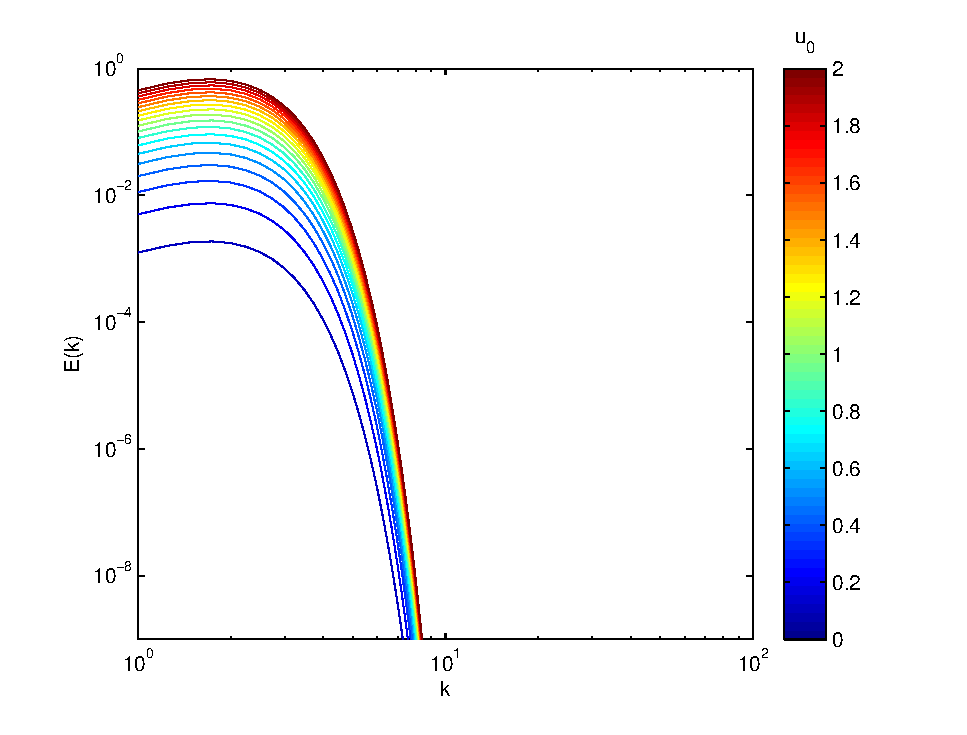
\includegraphics[width=0.48\textwidth]{Figures/eng_spr_u}
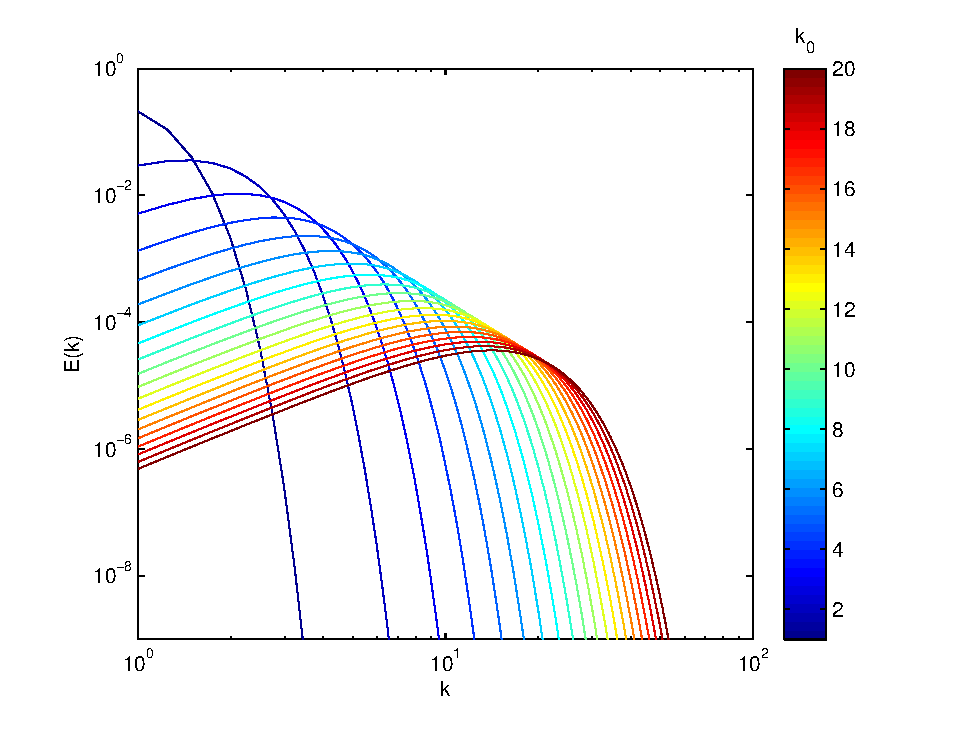
\includegraphics[width=0.48\textwidth]{Figures/eng_spr_k}
\caption{Initial energy spectrum with different parameters: left figure shows the energy spectrum with fixed $k_0 = 2.4$ while varing $u_0$ from $0m/s$ to $2m/s$, right figure shows the one with fixed $u_0 = 0.35m/s$ and varing $k$ from $1$ to $20$.\label{fig:eng_spr}}
\end{figure}

As for the external volume force, several solutions have been proposed in the literature, representing two main approaches. The first is to construct the force in Fourier space to keep a constant energy injection rate, and thus this method requires knowledge of Fourier-transformed velocities. In \cite{ghosal1995dynamic, Carati1995Representation}, the authors applied a force to the wavenumbers in the chosen shell, and guarantee a constant energy injection rate. The Ghosal's approach \cite{ghosal1995dynamic} can be simply formulated in the Fourier space: 
\begin{equation}
\mathbf{f}_e(\mathbf{k},t) = \epsilon_{in}\frac{\mathbf{u}(\mathbf{k},t)}
{\sum_{\mathbf{k}_f\in \kappa}|\mathbf{u}(\mathbf{k}_f,t)|^2}
\sigma_{\mathbf{k},\mathbf{k}_f}
\end{equation}
where $\mathbf{u}(\mathbf{k},t)$ is the Fourier-transformed velocity function, $\mathbf{k}_f$ is chosen from a subset of the wavenumber space $\kappa$ containing a few wavevectors, for example $(1,1,2)$ plus all permutations with respect to components and sign, $\epsilon_{in}$ is a constant input energy rate. $\delta_{k,k_f}$ is a delta function. Statistics stationary homogeneous turbulence can be obtained in DNS by forcing the low-wavenumber modes. There still exist many other approaches based on the Fourier transformation. For example, Sullivan and Chasnov attempted to maintaining constant kinetic energy in the lowest wavenumbers \cite{Sullivan1994Deterministic, Chasnov1991Simulation}. Eswaran and Pope in \cite{Eswaran1988} utilized a stochastic process to determine external forcing scheme. 

The second group is to evaluate the external force in physical space. This approach is attractive for applications since it does not require transformation to Fourier space and is easily integrated into physical-space numerical codes. Lundgren proposed a forcing function which is directly proportional to the velocity \cite{Lundgren2003Linearly}. Rosales studied the properties of this linear forcing scheme for isotropic turbulence, and showed the linearly forced system converges to a stationary state that does not depend on the spectral shape of the initial condition \cite{Rosales2005Linear}. The Lundgren's linear forcing scheme is determined with the following equation:
\begin{equation}
\vect{f}(\vect{x}, t) = \frac{\epsilon_{in}}{3u_{rms}^2}\vect{u}
\end{equation}
During the simulation, the root-mean-square velocity $u_{rms}$ is recalculated every time step while the energy injection rate $\epsilon_{in}$ is kept equal to a constant.
The cross section of the initial and stationary vorticity field is displayed in \Fig{fig:vort}.

\begin{figure}[!htbp]\centering
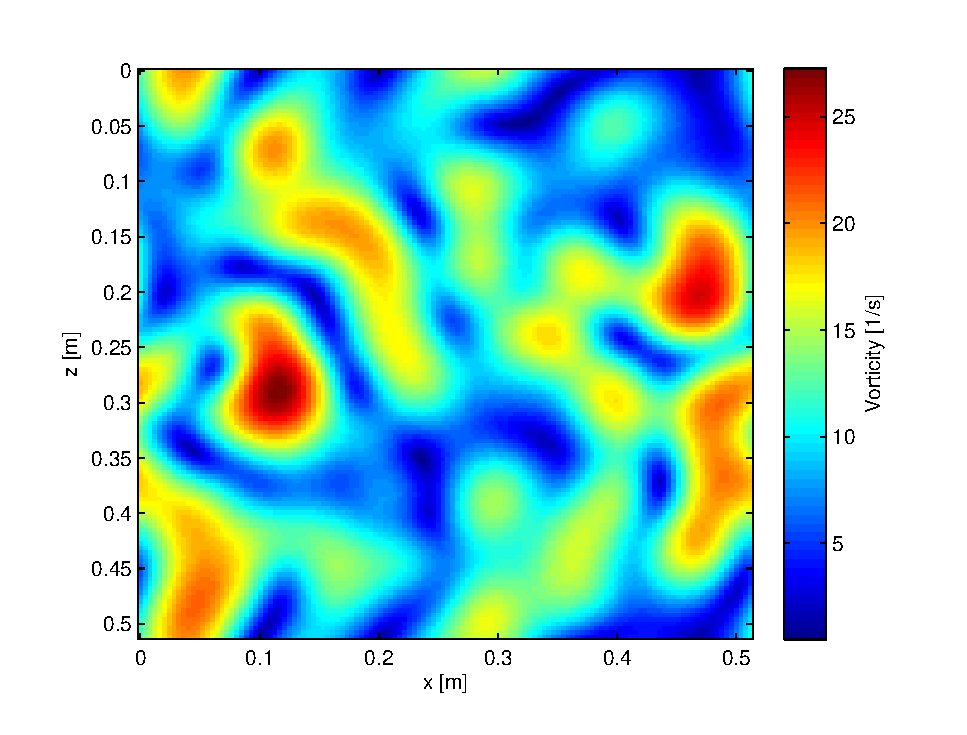
\includegraphics[width=0.45\textwidth]{Figures/vortex-0}
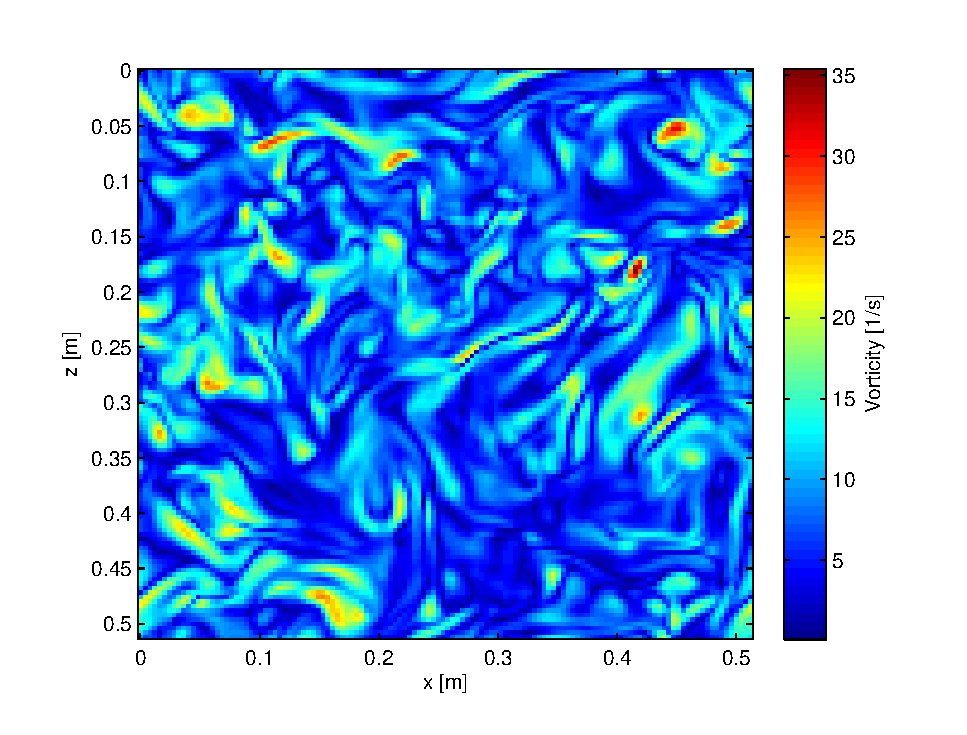
\includegraphics[width=0.45\textwidth]{Figures/vortex-1}

\caption{initial and final vorticity field ($1/s$) in x-z cross-sectional
plane for forced cases\label{fig:vort}}
\end{figure}

\section{Parallelism}
The numerical experiments for DNS of cloud entrainment mixing are carried out on the Linux cluster ``FASTER", named after the FASTER (Fast-Physics-System-Testbed and Research) project. The parallelization of this application involves three components: computation of fluid dynamics, computation of particles and runtime data analysis. The parallelization for the computation of fluid dynamics is done through domain decomposition and buffer extension. The computational domain is first uniformly divided into several partitions, and each partition has a buffer in each direction storing the information of its neighbor cells. The buffer is then updated every time step to provide the boundary information for the finite difference method. A typical $4\times 4\times 4$ partition of the computational domain is displayed in \Fig{fig:droplets_parallel}. 

\begin{figure}[!htbp] \centering
\includegraphics[width=0.6\textwidth]{Figures/droplets_parallel.jpg}
\caption{$4\times 4\times 4$ partitions of computational domain for the simulation of 
cloud droplets\label{fig:droplets_parallel}} 
\end{figure}

The computation of the particles is parallelized using a hybrid computing technique. After each time step, the particles with zero radius or exceeding the limits of the local domain are removed from the current partition or sent to its neighbors. The computation can be further accelerated using Open-MP or GPU technique within one time step. The combination of using MPI between computing nodes and shared memory computing inside a node results in a hybrid computing technique, which has become the mainstream of high performance computing.
In addition, the runtime data analysis also needs parallelization. For example, a parallel algorithm is required to calculate the mean and standard deviation of the droplets radius, temperature field, vapor mixing ratio field and velocity field. The calculation is first carried out in each processor by itself, and then aggregated to the answer using MPI reduce subroutine. However, since the size of the numbers $n$ is too large ($n = O(10^7)$ for cloud droplets and $n = O(10^6)$ for fields), simply summing a sequence of finite precision floating point numbers may accumulate the numerical error. To overcome this, we have applied the Kahan summation algorithm \cite{Kahan1965Pracniques}, in which the worst-case error bound is independent of $n$. Therefore, a large number of values can be summed with an error that only depends on the floating-point precision. 

Next chapter gives a detailed description of the numerical experiments and results. The data processing and analysis will also be presented.
\newpage{}
